% Figura Anexo II: la región de determinación del equilibrio en el plano de los coeficientes de la regla de TAYLOR
\documentclass[tikz,border=3pt]{standalone}
\usepackage[T1]{fontenc}
\usepackage[utf8]{inputenc}
\usepackage{amsmath}
\usetikzlibrary{arrows.meta,calc,positioning}
\begin{document}
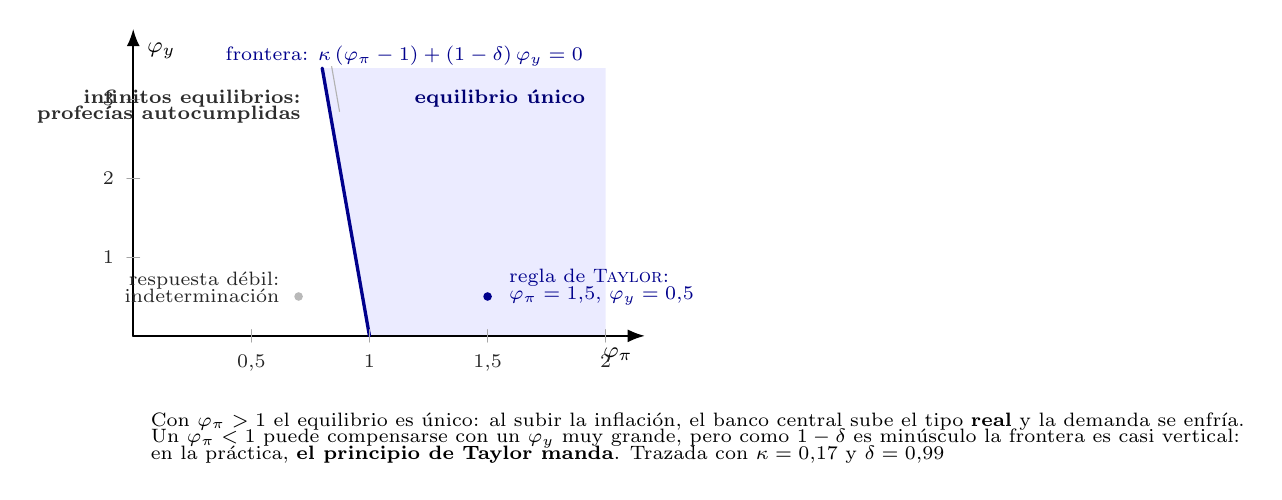
\begin{tikzpicture}[>={Latex[length=2.2mm]}, line cap=round, font=\footnotesize,
  eje/.style={->, thick},
  curva/.style={very thick},
  guia/.style={densely dashed, gray!80},
  pto/.style={circle, fill=black, inner sep=1.1pt}]
  % Region de determinacion (a la derecha de la frontera)
  \fill[blue!8] (2.40,3.40) -- (3.00,0) -- (6.00,0) -- (6.00,3.40) -- cycle;
  \draw[eje] (0,0) -- (6.5,0) node[below left=1pt]{$\varphi_{\pi}$};
  \draw[eje] (0,0) -- (0,3.9) node[below right=2pt]{$\varphi_{y}$};
  % Frontera: kappa(phi_pi - 1) + (1-delta) phi_y = 0
  \draw[curva, blue!55!black] (2.40,3.40) -- (3.00,0);
  \node[anchor=west, font=\scriptsize, blue!55!black, align=left] at (1.05,3.55)
    {frontera: $\kappa\left(\varphi_{\pi}-1\right)+\left(1-\delta\right)\varphi_{y}=0$};
  \draw[gray!60] (2.52,3.42) -- (2.62,2.85);
  % Marcas del eje
  \foreach \v/\t in {1.5/{$0{,}5$}, 3.0/{$1$}, 4.5/{$1{,}5$}, 6.0/{$2$}}{
    \draw[gray!70] (\v,-0.08) -- (\v,0.08);
    \node[font=\scriptsize, anchor=north, gray!30!black] at (\v,-0.12) {\t};
  }
  \foreach \v/\t in {1/{$1$}, 2/{$2$}, 3/{$3$}}{
    \draw[gray!70] (-0.08,\v) -- (0.08,\v);
    \node[font=\scriptsize, anchor=east, gray!30!black] at (-0.12,\v) {\t};
  }
  % Puntos
  \node[pto, fill=blue!55!black] (T) at (4.5,0.5) {};
  \node[anchor=west, font=\scriptsize, blue!55!black, align=left] at (4.65,0.62)
    {regla de \textsc{Taylor}:\\[-2pt]$\varphi_{\pi}=1{,}5$, $\varphi_{y}=0{,}5$};
  \node[pto, fill=gray!55] (I) at (2.1,0.5) {};
  \node[anchor=east, font=\scriptsize, gray!30!black, align=right] at (1.98,0.62)
    {respuesta débil:\\[-2pt]indeterminación};
  % Etiquetas de las zonas
  \node[font=\scriptsize\bfseries, blue!45!black, anchor=north west] at (3.45,3.25) {equilibrio único};
  \node[font=\scriptsize\bfseries, gray!35!black, anchor=north east, align=right] at (2.25,3.25) {infinitos equilibrios:\\[-2pt]profecías autocumplidas};
  \node[align=left, anchor=north west, font=\scriptsize] at (0.1,-0.85)
    {Con $\varphi_{\pi}>1$ el equilibrio es único: al subir la inflación, el banco central sube el tipo \textbf{real} y la demanda se enfría.\\[-2pt]Un $\varphi_{\pi}<1$ puede compensarse con un $\varphi_{y}$ muy grande, pero como $1-\delta$ es minúsculo la frontera es casi vertical:\\[-2pt]en la práctica, \textbf{el principio de \textsc{Taylor} manda}. Trazada con $\kappa=0{,}17$ y $\delta=0{,}99$};
\end{tikzpicture}
\end{document}
